\begin{figure}[!ht]
    \centering
    
    \begin{minipage}{.8\textwidth}
        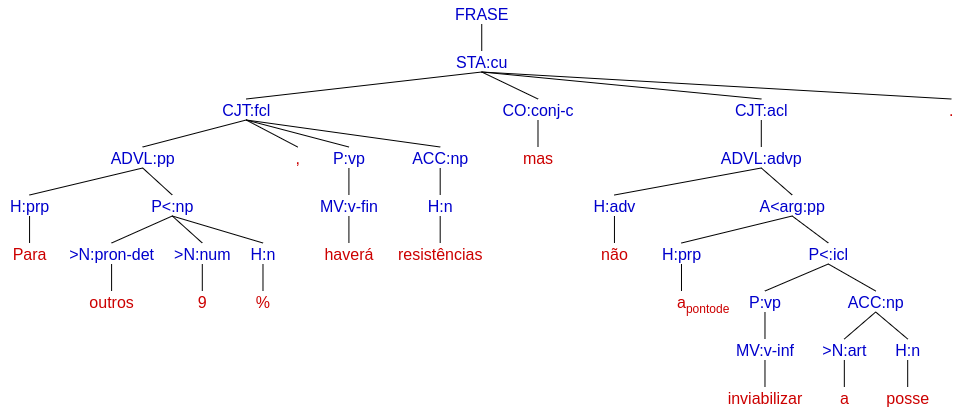
\includegraphics[width=\linewidth]{imagens/ec_bosque_perc_orig.png}
        \caption{árvore original}
    \end{minipage}
    % 
    \begin{minipage}{.8\textwidth}
        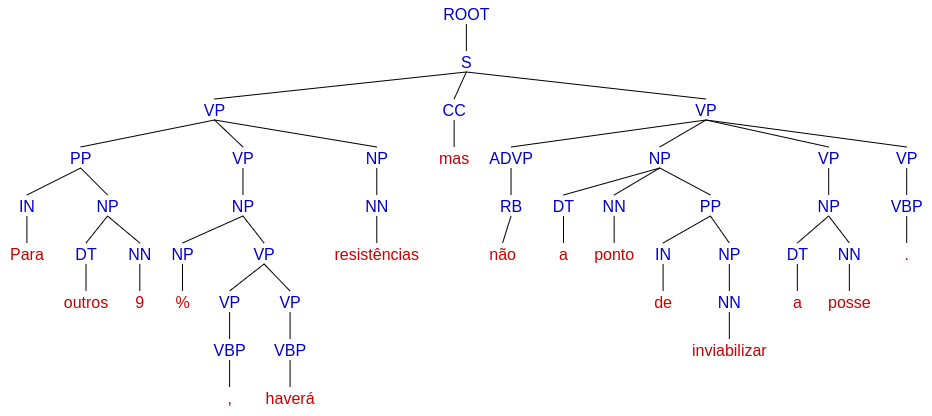
\includegraphics[width=\linewidth]{imagens/ec_bosque_perc_sp.png}
        \caption{árvore gerada pelo SP}
    \end{minipage}
    
    
    \caption[Estudo de caso BOSQUE - Sentença transduzida com sinal de porcentagem]{Estudo da sentença CF144-5, \textquote{ Para outros 9\%, haverá resistências mas não a ponto de inviabilizar a posse.}, que possui o símbolo de porcentagem. Note que, dessa vez, não há uma árvore do transdutor.}
    \label{fig:ec_bosque_perc_tree}
\end{figure}

